% ============================================================
% FraudLens · CPEC2026 实验教学案例稿（精简版 v2）
% 编译方式：XeLaTeX + BibTeX
% 参考文献：gbt7714-numeric + references_cpec.bib（13 篇）
% 页面：CPEC2026 模板（实验技术与管理版式）
% ============================================================
\documentclass[12pt,a4paper]{ctexart}

% ---- 匿名审稿条件编译：署名版 \anonfalse；投稿匿名版改 \anontrue ----
\newif\ifanon
\anonfalse

% ---- 中文断行 ----
\usepackage{fontspec}
\usepackage{xeCJK}
\setmainfont{Times New Roman}

% ---- 页面（CPEC2026 模板：上 3.5cm 给首页地脚留白）----
\usepackage[top=3.5cm, bottom=2.5cm, left=2.8cm, right=2.8cm]{geometry}

% ---- 行距 1.5 / 段首缩进 / 标题黑体（CPEC2026 模板规范）----
\usepackage{setspace}
\setstretch{1.5}
\usepackage{indentfirst}
\ctexset{
  section       = { format = \heiti\zihao{-3}\centering },
  subsection    = { format = \heiti\zihao{4} },
  subsubsection = { format = \heiti\zihao{-4} },
}

% ---- 图表 ----
\usepackage{graphicx}
\usepackage{booktabs}
\usepackage{array}
\usepackage{multirow}
\usepackage{caption}
\usepackage{float}
\captionsetup{font=small, labelfont=bf, labelsep=space}

% ---- 数学 ----
\usepackage{amsmath, amssymb}

% ---- 引用（GB/T 7714-2015 顺序编码制，gbt7714）----
\usepackage[numbers,sort&compress]{natbib}
\usepackage{gbt7714}
\usepackage{hyperref}
\hypersetup{
  colorlinks=true,
  linkcolor=black,
  citecolor=black,
  urlcolor=black
}

% ---- 矢量插图 ----
\usepackage{tikz}
\usetikzlibrary{positioning,fit,shadows,backgrounds,calc,arrows.meta}

\begin{document}

% ============================================================
% 题名区（手写，避免 ctexart \maketitle 产生空白首页）
% ============================================================

\begin{center}
  \centerline{\zihao{2}\heiti\bfseries 面向反诈团伙研判的 AI 赋能实验教学案例设计}\par\vspace{8pt}
  \ifanon
  \else
  {\zihao{4} 韩冬，吴燕波\textsuperscript{*}，徐伟}\\[2pt]
  {\zihao{5} （湖北警官学院~信息技术系，武汉~430034，中国）}
  \fi
\end{center}

\ifanon
\else
\vspace{4pt}
{\zihao{-5}\noindent
收稿日期：2026-XX-XX；基金项目：湖北省大学生创新创业训练计划项目（编号：S202611332001，徐伟、吴燕波共同指导）。\\
作者简介：韩冬（2005—），男，湖北，本科在读，主要研究方向为网络安全与人工智能反诈，E-mail：winterhdsec@163.com（电话：18202799140）。\\
徐伟（1978—），男，湖北，博士在读，副教授，研究方向为网络空间安全（网络入侵检测、物联网安全），E-mail：8073@hbpa.edu.cn。\\
通信作者：吴燕波（19xx—），女，湖北，硕士，副教授，研究方向为公安院校计算机与网络安全实践教学、网络安全与执法人才培养、警用智能装备应用，E-mail：240325743@qq.com（电话：13339993182）。}
\fi

% ------------------- 中文摘要（手写，确保铺满整行、无缩进）-------------------
\noindent\textbf{摘要：}在公安院校反诈实战课上，学生动手操作真实研判系统的机会有限，教师也缺少可直接落地的现成材料。本文以一套可运行的反诈研判原型系统 FraudLens 为载体，给出一份学生可一键复现的 AI 赋能实验教学案例。案例把系统的"串并案—扩线—反思"两级研判闭环改写成实训内容，按"研—训—评"模式组织四个递进实验环节，让学生在 Jupyter 环境里完成人机协同研判和算法边界认知训练，并配套带权重的评价量表与思政映射。区别于一般算法教学，本文以研判决策而非模型分析为核心，培养学生在 AI 辅助下做领域研判决策、人机协同与工程可信伦理的能力，为公安实战人才培养提供可复用的领域级实训素材。

\vspace{4pt}\noindent\textbf{关键词：}反诈教学；图神经网络；实验教学案例；研判决策；人机协同

\noindent\textbf{中图分类号：}TP393.08；TP18；G642 \qquad \textbf{文献标志码：}A

% ------------------- 英文题名 / 作者 / 摘要 -------------------
\vspace{1em}
\begin{center}
  {\heiti\Large Design and Exploration of an AI-Enabled Practical Teaching Case for Anti-Fraud}
  \ifanon
  \else
  \vspace{0.5em}
  {\normalsize HAN Dong, WU Yanbo\textsuperscript{*}, XU Wei}

  {\small Hubei University of Police, Department of Information Technology, Wuhan 430034, China}
  \fi
\end{center}

\begin{center}\textbf{Abstract:}\end{center}
\noindent To address the gap that students in anti-fraud practical teaching at police colleges can hardly operate a real investigation system hands-on while instructors lack ready-to-use, reproducible case material, this paper presents a reproducible, AI-enabled practical teaching case built on a working anti-fraud investigation prototype, FraudLens. The case reformulates the system's two-level investigation loop (case-level merging and account-level expansion) and its reflection orchestration into hands-on laboratory content, and organizes a four-lab progressive chain—case analysis, AI-assisted case linking, freeze-order ethical decision-making, and capability-boundary reflection—under a research–training–evaluation model. Guided by one-click reproducible baselines, students conduct human–AI collaborative investigation and algorithm-boundary reflection in a Jupyter environment, with weighted rubrics and ideological–ethical mapping throughout. Centered on investigative decision-making rather than model analysis, the case cultivates students' AI-assisted decision-making, human–AI collaboration, engineering trustworthiness, ethical responsibility, and boundary awareness, thereby providing a deployable domain-level training resource for police talent development.

\begin{center}\textbf{Key words:}\end{center}
anti-fraud; graph neural network; practical teaching case; investigative decision-making; human–AI collaboration

% ============================================================
% 1 引言
% ============================================================
\section{引言}

新工科建设要求计算机类人才具备 AI 赋能的实践能力和工程素养，把真实领域问题改写成可复现的实践教学案例，是提升学生实战能力的一条可行路径~\cite{edu_liqingyong2024,edu_zhangjin2024}。但现有计算机实践教学案例大多围绕通用编程和单门课程~\cite{edu_zhangjin2024}，领域级实战研判（比如涉网犯罪智能研判）的可复现案例仍属稀缺~\cite{edu_xiangga2022}。在公安院校，这一问题更突出：反诈实战课上，学生长期只能听案例、看演示，很难亲手操作一套真实的研判系统；教师也缺少既适合课堂、又能让学生复现的现成材料。

本文是一篇面向反诈实战教学的\textbf{实验教学案例设计}，不是算法研究论文，重点在于怎样把 FraudLens 这个可运行的反诈研判原型系统变成学生可动手、教师可直接落地的实训载体，算法本身的实现细节不在讨论范围内。按工程教育对复杂工程问题的通行界定（要求深入工程原理分析、多因素冲突、建立抽象模型、非常规方法可解、利益不一致、含多个关联子问题）~\cite{edu_jiangzongli2016,edu_xiangga2022}，反诈团伙研判可以逐条对应：资金拓扑和话术文本构成多源异构数据，需建立图抽象模型；团伙反侦查行为带来多因素冲突；冻卡决策涉及利益与规范权衡；研判流程包含数据建模、表示学习、系统编排与可信决策等多个关联子问题。以反诈团伙研判为载体的实训，能让学生在真实问题里综合运用图建模、深度表示学习、系统编排与工程可信设计；教学落脚点是让学生在 AI 辅助下做出领域研判决策、并对算法能力边界保持审慎认知，独立"解决复杂工程问题"不在实训要求之内。

按这一思路，本文以可运行的反诈团伙研判原型系统 FraudLens 为载体，把"案件级串并案 + 账户级扩线"两级研判闭环与反思编排整合为实训内容，构建一份可复现的"研—训—评"一体化教学案例。主要工作如下：
\begin{enumerate}
  \item 给出一套可落地的 AI 辅助研判决策实训载体。FraudLens 两级研判系统（"案件级串并案 + 账户级扩线"闭环，由 LangGraph StateGraph~\cite{langgraph2024} 编排"规划 $\to$ 预处理 $\to$ 分析 $\to$ 聚类 $\to$ 反思"工作流），技术栈覆盖图建模、异构注意力、系统编排与工程可信，可作为学生"研"的对象逐层复现。
  \item 提出"研—训—评"一体化的实训模式。按"案情分析 $\to$ 工具辅助串并案 $\to$ 冻卡决策与伦理权衡 $\to$ 边界认知与反思"设计 4 环节递进实验链（第~5~节），以研判决策为核心活动，配套带权重的评价量表与思政/伦理映射。
  \item 提供可复现实验与科学边界认知训练。能力基线（HAN 困难场景 F1=0.9154、反思闭环增益 +0.5125、账户级扩线将团伙 F1 由盲扫约 0.002 提升至约 0.71）全部可一键复现\footnote{文中能力基线/消融数据由系统仓库 \texttt{backend/gnn/eval\_framework.py} 复现（结果见 \texttt{backend/gnn/eval\_full\_results.json}，合成数据 10 seeds，mean$\pm$std）；AMLSim 账户级扩线数据由 \texttt{backend/gnn/pathb\_final\_push.py} 复现（k-core 与短有向环基线，结果见 \texttt{backend/gnn/pathb\_final\_push\_results.json}，盲扫基线见 \texttt{backend/gnn/blind\_sweep\_results.json}），全部随系统开放、可在本地 Jupyter 中复现。}；同时诚实量化反诈 GNN 的增量边界（合成 $\neq$ 真实、盲扫全败、不构成真实警务验证），引导学生建立对模型能力的审慎认知。
\end{enumerate}

文中能力基线数据（如 HAN 困难场景 F1、反思闭环增益、扩线召回）只作为实训可复现对象的佐证，不代表真实警务场景的已验证成效；教学成效的课堂实证评估属下一阶段工作。

% ============================================================
% 2 相关工作
% ============================================================
\section{相关工作}

\subsection{反诈团伙检测技术}

反诈检测经历了从规则到图神经网络的演进：基于规则的串并案依赖办案经验、难以规模化；浅层聚类无法建模账户间复杂关联；图神经网络（GNN）~\cite{hamilton2017graphsage} 虽能利用图结构，欺诈场景亦已考虑伪装节点与拓扑~\cite{dou2020caregnn}，但同构 GNN 难以同时建模案件、账户、违法者等多类实体及其关系，本文因此采用异构注意力网络（HAN）~\cite{wang2019han}。从教学角度看，这条技术演进线本身即"数据建模 $\to$ 表示学习 $\to$ 工程决策"的完整教材。

\subsection{人工智能赋能实验教学}

以大语言模型为代表的人工智能正加速融入计算机实践教学：李清勇等~\cite{edu_liqingyong2024} 探讨了通用大模型在实践教学中的角色定位，张金等~\cite{edu_zhangjin2024} 构建了基于通用大模型的系统创新实验。但现有案例大多围绕通用编程和单门课程，面向领域级实战研判的可复现案例仍属稀缺~\cite{edu_xiangga2022}。本文据此把 FraudLens 设计为可复现实验案例，支撑学生从数据建模到科学边界认知的递进训练。

% ============================================================
% 3 系统概览
% ============================================================
\section{实训载体：FraudLens 系统概览}
\label{sec:arch}

FraudLens 是一套可运行的反诈团伙研判原型系统（图~\ref{fig:arch}），覆盖数据建模、表示学习、系统编排与工程可信的完整技术链，对应实训所需的知识与能力结构，可作为"研"的对象。系统逻辑上构成两级研判闭环：案件级串并案（一级）以 HAN 在案件异构图上聚合同伙案件，账户级扩线（二级）在给定线索锚点后于账户交易子图上还原资金链路；一级输出的关键账户可直接作为二级扩线的锚点，契合真实反诈工作流。对实训而言，这套闭环覆盖了从数据到决策的完整链路，学生可沿两级闭环逐段复现。

\begin{figure}[htbp]
  \centering
  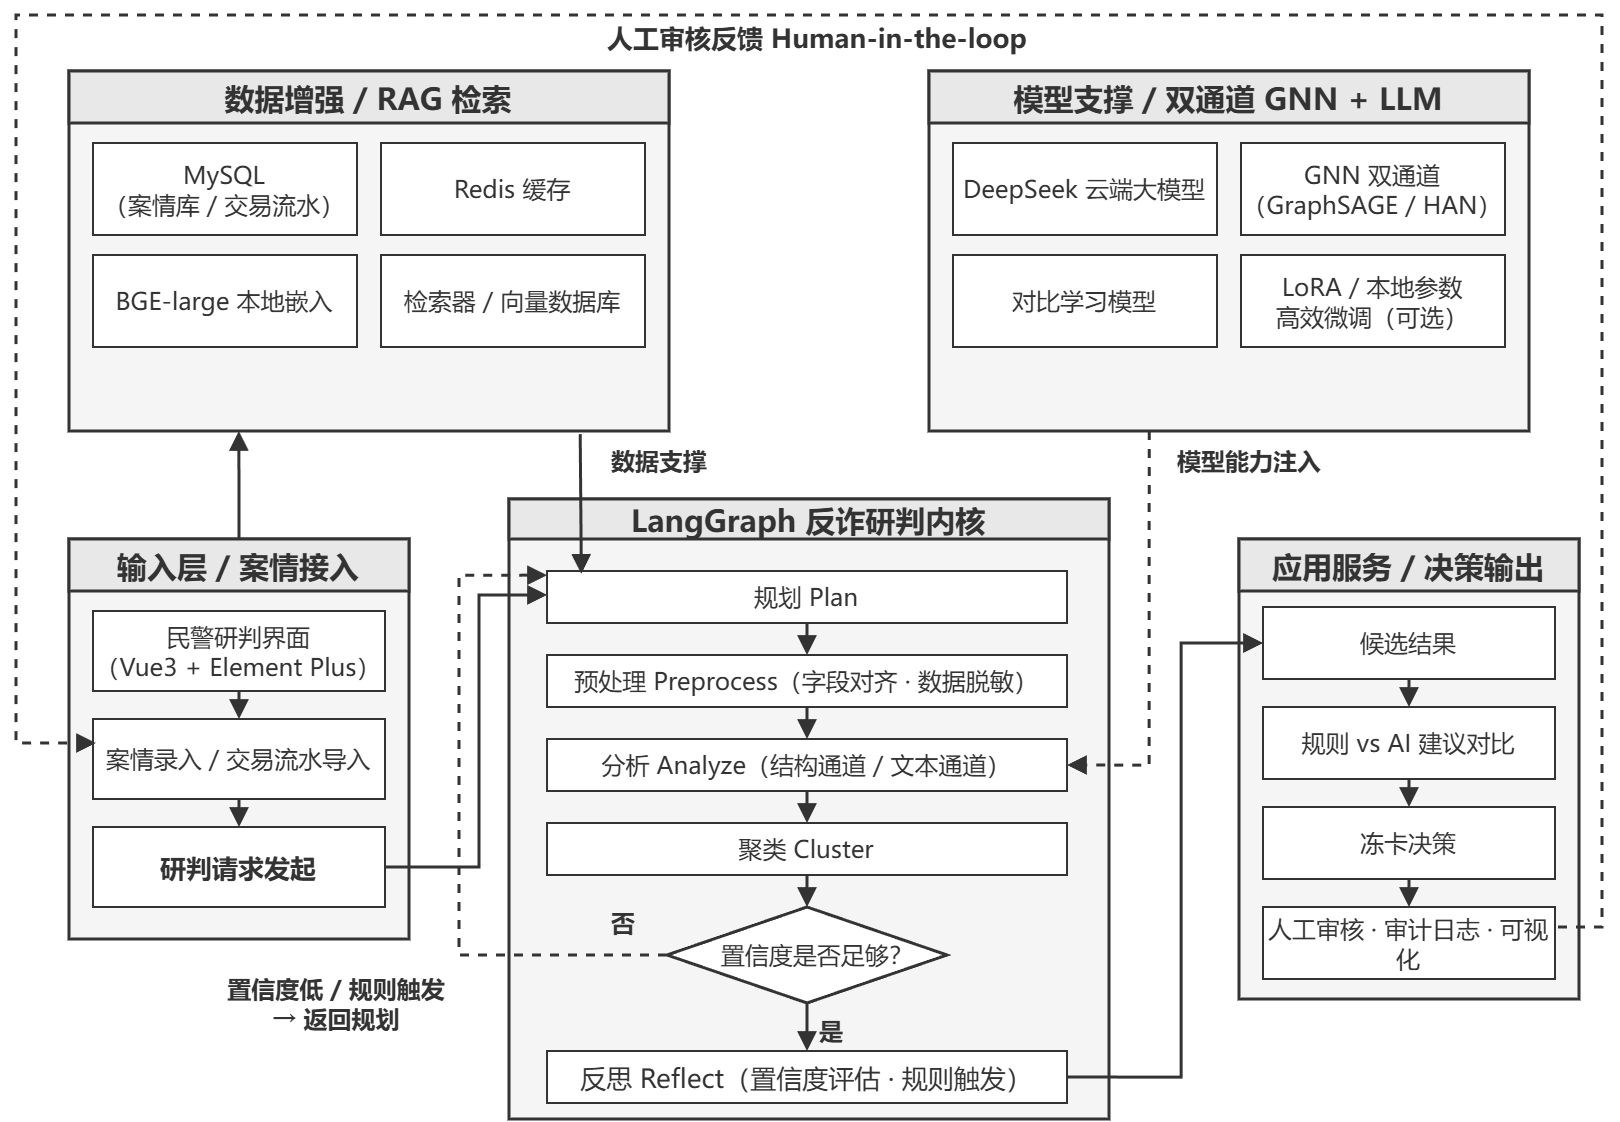
\includegraphics[width=\linewidth]{fig_arch.png}
  \caption{FraudLens 系统总体架构}
  \label{fig:arch}
\end{figure}

为降低上手门槛，实训以研判决策为核心，不要求学生理解图神经网络内部原理；全部模块均提供预计算结果供学生交互使用。系统的技术构成可概括为四点：异构双通道融合——以 HAN~\cite{wang2019han} 融合"结构通道（金额加权交易图）"与"文本通道（本地 BGE 语义嵌入）"，支撑案件级团伙聚类；多智能体反思闭环——由 LangGraph~\cite{langgraph2024} 驱动"规划 $\to$ 预处理 $\to$ 分析 $\to$ 聚类 $\to$ 反思"工作流，反思节点在聚类质量不达标时经条件边回连触发真实重算~\cite{shinn2023reflexion}；经验加权置信度门控——以团伙规模、涉案金额、关联账户数、资金回流四因子加权给出冻卡建议置信度；工程可信——实现 RBAC 鉴权、双表审计、多级降级链与"数据不出域"，契合公安院校数据合规要求。这些技术细节不是本文讨论重点，本文只把它们作为实训"研"的对象。

为直观呈现学生操作 FraudLens 与之协同研判的过程，图~\ref{fig:workflow} 给出学生实验流程与系统响应机制：学生以四环节实验链为单位向系统输入案情与参数，系统经预处理、语义嵌入与图构建形成研判对象，由 LangGraph 多智能体状态图完成"规划—预处理—分析—聚类—反思"，输出候选结果供学生做人机协同决策；全程审计日志与加权评价量表支撑"研—训—评"闭环。

\begin{figure}[htbp]
  \centering
  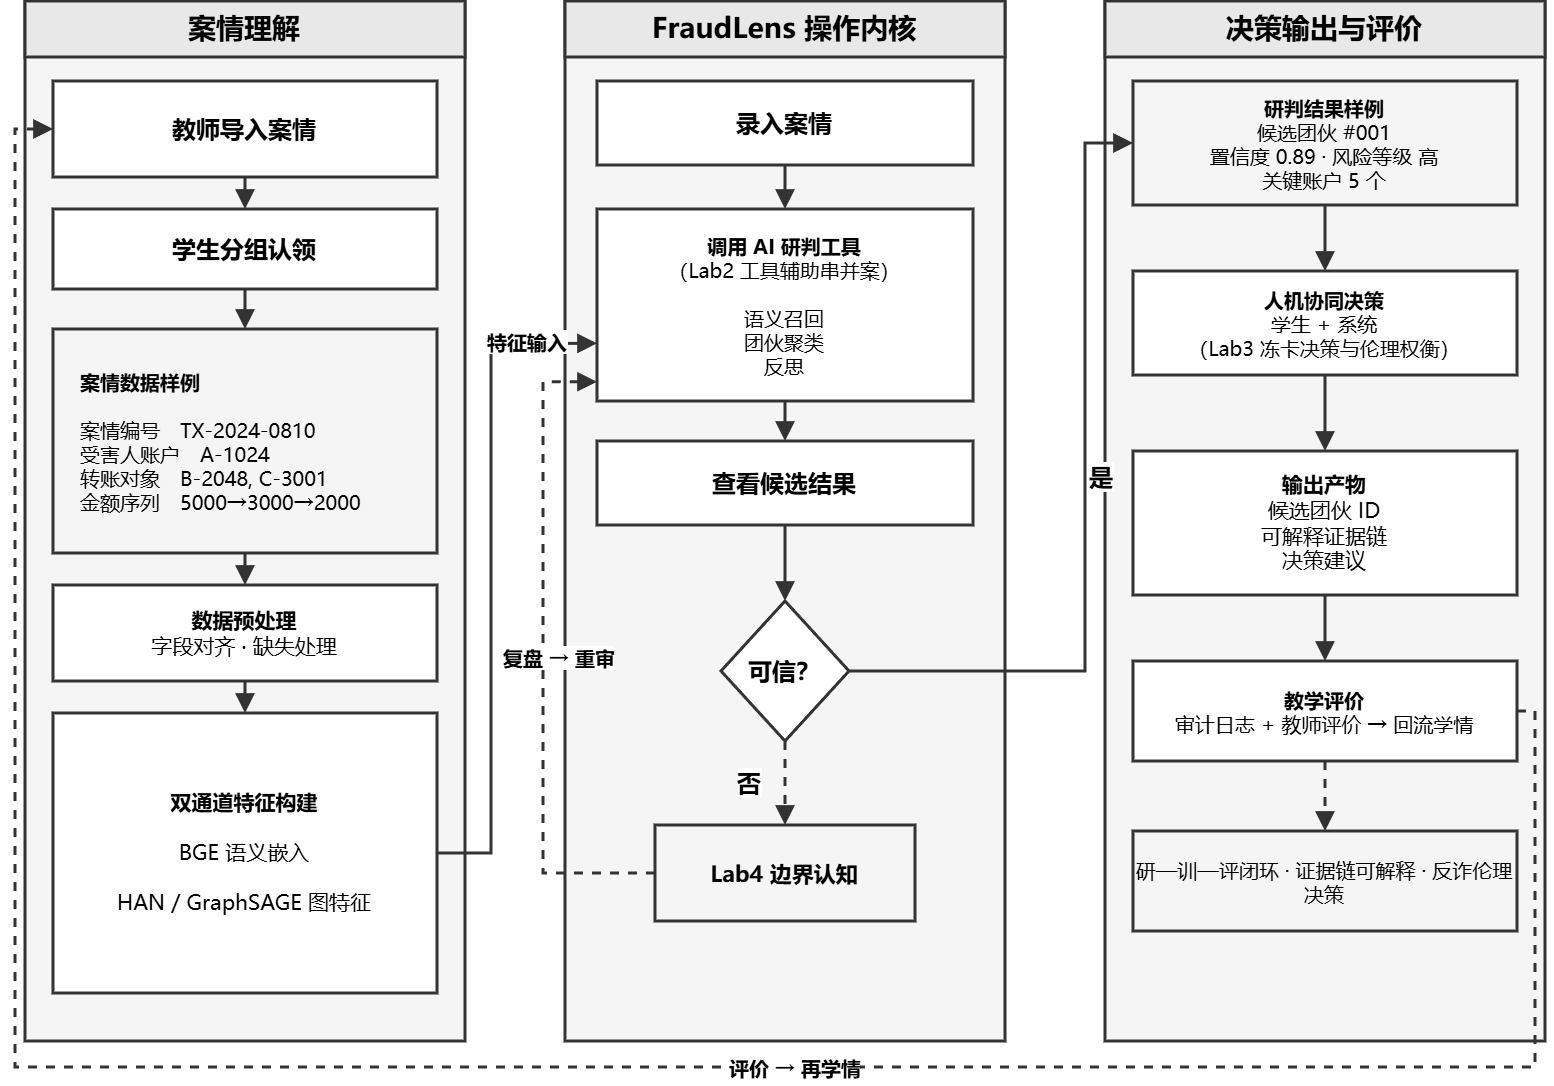
\includegraphics[width=\textwidth]{fig_workflow.png}
  \caption{学生实验流程与系统响应机制（示意图）}
  \label{fig:workflow}
\end{figure}

% ============================================================
% 4 实训可复现性与能力基线
% ============================================================
\section{实训可复现性与能力基线}

本节给出 FraudLens 两级研判能力的可复现性与能力边界的三层实验验证，作为实训的科学基线：（1）合成数据能力基线与消融——在受控合成案情上确认模型判别水平，定位反思闭环与异构图建模各自的贡献；（2）AMLSim 账户级扩线外部验证——在真实规模的公开反洗钱基准上考察无监督扩线的能力上限；（3）Elliptic 跨数据集边界对照——援引公开基准结果，说明方法对无金额/时序的纯拓扑交易图不迁移。三层验证共同支撑"可复现、有上限、边界诚实"的实训基调，全部数据随系统开放、可一键复现。

实训以可复现为设计前提：合成案情数据集随系统开放，全部实验提供一键复现脚本；HAN 采用无标签预训练，不依赖人工团伙标注；外部验证所用 Elliptic~\cite{weber2019elliptic}、AMLSim~\cite{weber2018amlfirstlook} 均为公开数据，学生可在本地完整复现。能力基线中的合成数据不等于真实警务数据，这一边界本身会被放入实训 Lab4 作为教学内容。

\subsection{能力基线与消融}

表~\ref{tab:baselines} 报告合成数据（10 随机种子均值）下的能力基线。HAN 在困难（Hard）场景 F1=0.9154，比同构 GraphSAGE（Hard F1=0.3043，因无法建模多类型实体关系发生塌缩）高出很多，这一对比直接成为实训 Lab2"为何需要 AI 辅助"的教学素材。消融显示，反思闭环只作用于未收敛的失败场景：其缺失使失败场景 F1 由 0.8353 跌至 0.3228（增益 +0.5125），说明反思闭环对该类场景是不可或缺的；关闭 GNN 退化为 Louvain 社区发现，Hard F1 由 0.9154 降至 0.8616，说明异构图建模对困难场景同样是必要的。

\begin{table}[htbp]
  \centering
  \caption{能力基线与消融（合成数据，10 seeds mean$\pm$std）}
  \label{tab:baselines}
  \begin{tabular}{lccp{3.2cm}}
    \toprule
    方法/配置 & Clean F1 & Hard F1 & 备注 \\
    \midrule
    \textbf{HAN（本文）} & \textbf{1.0000$\pm$0.0000} & \textbf{0.9154$\pm$0.1214} & 异构注意力融合 \\
    GraphSAGE & 0.4061$\pm$0.2127 & 0.3043$\pm$0.0000 & Hard 塌缩（同构局限） \\
    Louvain（降级） & 0.8884$\pm$0.0911 & 0.8616$\pm$0.0874 & 关闭 GNN 的社区发现 \\
    w/o 反思闭环 & — & — & 失败场景 F1 由 0.8353 跌至 0.3228 \\
    \bottomrule
  \end{tabular}
  \par\vspace{1.5\baselineskip}
  \begin{minipage}{\textwidth}
  \footnotesize
  \setstretch{1.15}
  \noindent 注：Clean 场景无跨团伙干扰（cross=0.0），仅验证模型基本学习能力，不代表真实场景预期。反思闭环仅作用于失败场景的自动降级重算，不改变已收敛场景均值，故 w/o 反思的 Hard F1 以“—”表示。
  \end{minipage}
\end{table}

\subsection{账户级扩线外部验证（AMLSim）}
\label{sec:amlsim}

为验证账户级扩线（二级闭环）在真实规模公开图上的能力边界，本节在 AMLSim~\cite{weber2018amlfirstlook} 反洗钱基准（43,614 账户 / 1,305 个洗钱环，含账户级环真值）上报告无监督扩线结果：给定嫌疑账户锚点，于账户交易图上做 k=1 跳扩线，子图规模约 2,748 节点（环占比约 0.55），全部方法零标签、纯无监督。表~\ref{tab:amlsim} 显示，盲扫（全网无锚点）几乎失效（F1$\approx$0.002），印证"盲扫 vs 扩线"瓶颈；扩线设定下，k-core 核心子图（kmin=2）以无监督方式将团伙识别 F1 提升至约 0.71（召回 0.91），短有向环检测将资金环识别 F1 提升至约 0.62。该结果不宣称真实警务验证——AMLSim 为公开合成基准；其适用边界明确：只适用于含金额/时序的账户交易图，对纯拓扑交易图（Elliptic，无金额时序）不迁移。"无监督有上限、标注能破但不稳"的结论，正是实训 Lab4 的数据素材\footnote{本节 AMLSim 扩线数据由系统仓库 \texttt{backend/gnn/pathb\_final\_push.py} 复现（k-core 与短有向环基线，结果见 \texttt{backend/gnn/pathb\_final\_push\_results.json}；盲扫基线见 \texttt{backend/gnn/blind\_sweep\_results.json}），学生可在本地直接运行。}。

\begin{table}[htbp]
  \centering
  \caption{AMLSim 账户级扩线无监督基线（锚点 k=1 跳，零标签）}
  \label{tab:amlsim}
  \begin{tabular}{lcccc}
    \toprule
    任务 & 方法 & Precision & Recall & F1 \\
    \midrule
    团伙识别 & 盲扫（无锚点） & — & — & $\approx$0.002（失效） \\
    团伙识别 & k-core 核心子图（kmin=2） & 0.58 & 0.91 & \textbf{0.71} \\
    资金环识别 & 短有向环检测（L$\le$8） & 0.63 & 0.61 & \textbf{0.62} \\
    \bottomrule
  \end{tabular}
  \par\vspace{1.5\baselineskip}
  \begin{minipage}{\textwidth}
  \footnotesize
  \setstretch{1.15}
  \noindent 注：AMLSim 为 IBM 公开合成反洗钱基准，含账户级环真值；全部方法零标签纯无监督，不构成真实警务数据验证。k-core 召回 0.91 但候选占子图约 85\%，故 precision 受限——这正是无监督上限的结构性原因（详见~\S\ref{sec:lab4} Lab4）。
  \end{minipage}
\end{table}

上述两层验证（合成数据能力基线与消融、AMLSim 账户级扩线）均由本文在系统仓库中实地复现；为进一步标定"无监督有上限"的边界，本文另直接援引 Elliptic 公开基准上的报告结果（HAN F1$\approx$0.016），说明当前方法对缺少金额/时序的纯拓扑交易图不迁移。三层结果共同成为 Lab4"真实数据上所有方法都接近失败"的教学对照，让学生在动手实验前就对模型能力边界有较清醒的预期。

% ============================================================
% 5 实训教学设计
% ============================================================
\section{实训教学设计}
\label{sec:teaching}

FraudLens 所覆盖的技术栈——异构图谱建模、双通道语义融合、多智能体反思编排、可解释门控决策——和"新工科"对 AI 赋能实践能力与工程素养的要求能够对应。本节给出把它转化为可复现实训教学案例的设计方案，供"人工智能安全""图数据挖掘"及相关专业课程参考。以下为基于系统真实能力的\textbf{教学案例设计}，课堂实施与成效以实际开课情况为准。

\subsection{学情分析与课程衔接}

本案例面向公安院校信息技术、网络安全与侦查相关专业的本科生（建议大二下至大三上）实施。学生已修 Python 程序设计、数据结构与数据库等课程，具备基本图论概念与编程调试能力，但一般没有图神经网络与多智能体的先验~\cite{edu_zhangjin2024}；这两部分不作先修要求，只以黑箱工具形式参与，确保实训不依赖高阶先验。课程对接《人工智能安全》《图数据挖掘》等。据此，实训以\textbf{研判决策}为核心活动：图神经网络作为学生交互的黑箱工具，只要求学生理解"系统给出什么结果、可信到什么程度、何时该信、何时不该信"，而不要求掌握模型内部机理。全部实验以 Jupyter Notebook 为载体，系统研判结果预烘焙供学生对比分析。

\subsection{教学理念与“研—训—评”一体化模式}

本节以\textbf{“研—训—评”一体化}模式组织实训（图~\ref{fig:mode}）：以真实 FraudLens 系统为"研"的对象，以四环节递进实验链为"训"的载体，以过程+产物双轨评价及思政/伦理素养观测为"评"的手段，并以可复现实验、诚实边界认知与课程思政作为全程支撑。该模式把技术内容组织为"研究—训练—评价"的教学闭环，让育人主线不被技术细节盖过。

上述"研—训—评"在\textbf{教学设计层面}已构成完整的闭环（目标—活动—评价—反思）；\textbf{实证成效层面}的闭环，即学生实际走完四环节、测出能力提升并反馈改进，将在 2026 年秋季学期课程实施后闭合。当前稿以设计论证与可复现能力基线为支撑，教学成效以实际开课情况为准。

\begin{figure}[htbp]
  \centering
  \begin{tikzpicture}[
    band/.style={draw=black, rounded corners=4pt, minimum width=13.4cm,
      minimum height=0.85cm, align=center, font=\small},
    col/.style={draw=black, rounded corners=4pt, minimum width=3.6cm,
      minimum height=7.0cm, font=\small},
    colhdr/.style={draw=black, rounded corners=2pt, minimum width=3.6cm,
      minimum height=0.55cm, align=center, font=\small\bfseries,
      text width=3.2cm, inner sep=2pt},
    box/.style={draw=black, rounded corners=2pt, fill=white,
      minimum width=3.3cm, minimum height=0.85cm, align=center, font=\footnotesize,
      inner sep=4pt, text width=3.0cm},
    lbl/.style={font=\small\bfseries},
    arrow/.style={->, >=stealth, thick}
  ]
    \node[band, fill=white] (GOAL) at (0,4.3)
      {\textbf{目标层：培养 AI 辅助研判决策与算法边界认知}};
    \node[col, fill=white] (YAN) at (-4.7,0) {};
    \node[col, fill=white] (XUN) at (0,0) {};
    \node[col, fill=white] (PING) at (4.7,0) {};
    \node[colhdr, fill=white] at ([yshift=-0.5cm]YAN.north) {研 · 剖析真实系统};
    \node[colhdr, fill=white] at ([yshift=-0.5cm]XUN.north) {训 · 四环节实验链};
    \node[colhdr, fill=white] at ([yshift=-0.5cm]PING.north) {评 · 过程+产物};
    \node[box] at ([yshift=1.475cm]YAN.center)
      {\textbf{以系统为研对象}\\\footnotesize 可运行原型系统};
    \node[box] at ([yshift=-0.325cm]YAN.center)
      {\textbf{复现与剖析}\\\footnotesize 沿两级闭环逐段复现};
    \node[box] at ([yshift=-2.125cm]YAN.center)
      {\textbf{技术构成拆解}\\\footnotesize 图建模·表示·编排};
    \node[box] at ([yshift=1.835cm]XUN.center)
      {\textbf{Lab1 案情分析}\\\footnotesize 研判流程·认识系统};
    \node[box] at ([yshift=0.395cm]XUN.center)
      {\textbf{Lab2 串并案}\\\footnotesize 人工 vs AI 对比};
    \node[box] at ([yshift=-1.045cm]XUN.center)
      {\textbf{Lab3 冻卡决策}\\\footnotesize 门控·伦理权衡};
    \node[box] at ([yshift=-2.485cm]XUN.center)
      {\textbf{Lab4 边界反思}\\\footnotesize 失败·诚实反思};
    \node[box] at ([yshift=1.475cm]PING.center)
      {\textbf{过程评价 40\%}\\\footnotesize 任务完成度·协作};
    \node[box] at ([yshift=-0.325cm]PING.center)
      {\textbf{产物评价 60\%}\\\footnotesize 报告·代码·答辩};
    \node[box] at ([yshift=-2.125cm]PING.center)
      {\textbf{素养观测}\\\footnotesize 思政与伦理映射};
    \node[band, fill=white] (SUP) at (0,-4.3)
      {\textbf{支撑：可复现实验 + 诚实边界认知 + 课程思政与伦理}};
    \draw[arrow] ([xshift=-4.7cm]GOAL.south) -- (YAN.north);
    \draw[arrow] (GOAL.south) -- (XUN.north);
    \draw[arrow] ([xshift=4.7cm]GOAL.south) -- (PING.north);
    \draw[arrow] ([xshift=-4.7cm]SUP.north) -- (YAN.south);
    \draw[arrow] (SUP.north) -- (XUN.south);
    \draw[arrow] ([xshift=4.7cm]SUP.north) -- (PING.south);
  \end{tikzpicture}
  \caption{“研—训—评”一体化反诈实训模式框架}
  \label{fig:mode}
\end{figure}

\subsection{四环节递进实验链}
\label{sec:stages}

实训以四环节递进实验链为主线（图~\ref{fig:stages}）：四个 Lab 从案情分析到边界反思逐级递进，每个 Lab 锚定 FraudLens 的真实模块，以\textbf{研判决策}为核心活动。系统研判结果预烘焙为 JSON/NumPy 数组，学生打开 notebook 执行 Run All 即可获得案情数据与系统分析结果，教学时间用于决策、对比与反思。表~\ref{tab:stages} 给出各 Lab 的课时分配、核心任务、对应能力目标与训练产出。

\begin{figure}[H]
  \centering
  \begin{tikzpicture}[
    stage/.style={draw=black, rounded corners=4pt, minimum width=2.7cm,
      minimum height=4.0cm, align=center, font=\small, inner sep=4pt,
      text width=2.5cm},
    arrow/.style={->, >=stealth, thick, shorten >=2pt, shorten <=2pt}
  ]
    \node[stage, fill=white] (S1) at (-5.25,0)
      {\textbf{Lab1}\\\textbf{案情分析与研判流程}\\[2pt]分析案情·认识系统\\[2pt]\footnotesize 研判分析能力};
    \node[stage, fill=white] (S2) at (-1.75,0)
      {\textbf{Lab2}\\\textbf{工具辅助串并案}\\[2pt]人工 vs AI 对比\\[2pt]\footnotesize 人机协同能力};
    \node[stage, fill=white] (S3) at (1.75,0)
      {\textbf{Lab3}\\\textbf{冻卡决策与权衡}\\[2pt]门控调参·伦理角色扮演\\[2pt]\footnotesize 决策与伦理能力};
    \node[stage, fill=white] (S4) at (5.25,0)
      {\textbf{Lab4}\\\textbf{边界认知与反思}\\[2pt]系统失败·诚实反思\\[2pt]\footnotesize 边界认知能力};
    \draw[arrow] (S1.east) -- (S2.west);
    \draw[arrow] (S2.east) -- (S3.west);
    \draw[arrow] (S3.east) -- (S4.west);
  \end{tikzpicture}
  \caption{四环节递进实验链及其与系统模块对应}
  \label{fig:stages}
\end{figure}

\begin{table}[H]
  \centering
  \caption{四环节递进实验链——课时分配、核心任务与训练产出}
  \label{tab:stages}
  \begin{tabular}{cp{1.4cm}p{3.0cm}p{3.2cm}p{2.4cm}}
    \toprule
    Lab & 时长 & 核心任务 & 对应能力/系统模块 & 训练产出 \\
    \midrule
    1 & 4 课时 & 分析案情，认识研判流程 & 案情分析能力·\S\ref{sec:arch} 系统概览 & 案情分析报告 \\
    2 & 4 课时 & 人工串并案 vs 系统结果 & 人机协同·双通道 HAN+反思闭环 & 对比报告 \\
    3 & 4 课时 & 门控调参，冻卡决策角色扮演 & 决策与伦理·置信度门控 & 伦理分析报告 \\
    4 & 4 课时 & 系统失败场景与诚实反思 & 科学边界认知·外部验证 & 边界反思总结 \\
    \bottomrule
  \end{tabular}
  \par\vspace{1.5\baselineskip}
  \noindent{\scriptsize 注：课前预习 2 课时（\texttt{pip install} + 数据集下载，不计入课内学时）。课堂导入与总结内嵌于各 Lab，课内总计 16 学时。}
\end{table}

\subsubsection{Lab1：案情分析与研判流程}

\textbf{教学目标}：理解反诈案件的数据结构与研判流程。学生拿到一份合成案情（含受害者陈述、账户流水、通话记录、涉案金额），以办案人员视角分析：涉及哪些账户？钱怎么转的？哪个环节是关键节点？然后系统展示如何把同一案件建模为异构图可视化（案件—账户—手机号—类型—城市）。收尾讨论："如果只用传统逐笔查账方式，你会漏掉什么？"

\subsubsection{Lab2：工具辅助串并案}

\textbf{教学目标}：体验 AI 辅助串并案的价值与局限，建立"人机协同"意识。学生先\textbf{人工}判断"哪几个案子可能是同一伙人干的"，再运行系统看聚类结果。对比一下人和系统各自找到的——系统发现了人漏掉的多跳关联，人也可能发现系统漏掉的（基于办案经验而非数据特征的关联）。AI 能看到人看不到的结构关联，但也有盲区，\textbf{AI 是辅助工具而非替代}。

\subsubsection{Lab3：冻卡决策与伦理权衡}

\textbf{教学目标}：在真实决策压力下理解技术—伦理权衡。学生调整置信度门控阈值，观察阈值变化如何影响冻卡建议数量。\textbf{角色扮演}："如果阈值设高了，3 个无辜者的账户被冻结；如果设低了，团伙今晚转移资金。"学生记录决策理由并讨论："算法建议冻，但谁来承担后果？"冻卡不是单纯的技术问题，它本质上是伦理问题。

\subsubsection{Lab4：边界认知与诚实反思}
\label{sec:lab4}

\textbf{教学目标}：建立对 AI 研判工具能力边界的认知。学生观察同构 GNN 基线（GraphSAGE）在困难场景塌缩（F1 由约 0.41 跌至 0.30），而异构 HAN 保持 0.9+；再读 AMLSim 盲扫 F1$\approx$0.002、Elliptic HAN F1$\approx$0.016——\textbf{真实数据上所有方法都接近失败}。引入"扩线"概念：给定锚点 $\to$ 只分析 k 跳邻居 $\to$ 无监督拓扑方法将团伙识别 F1 由盲扫 0.002 提升至约 0.71、资金环识别约 0.62，无需任何标签，纯无监督就能显著恢复团伙与资金链；但这一增益只适用于含金额/时序的账户交易图，少量标注校准带来的进一步增益并不稳定。教学要点：反诈 GNN 的瓶颈不在算法设计，而在"盲扫 vs 扩线"的任务设定与无监督方法的适用边界。学生写 300 字反思："作为未来的警务技术使用者，你在什么情况下会信任这个系统？什么情况下不会？"

\subsection{考核方式设计}

考核采用"过程+产物"双轨（表~\ref{tab:rubric}），评价的核心不是指标最大化，而是学生对"系统能力与局限"的如实把握——既看到 AI 辅助研判的价值，也理解它在真实场景中的局限，这一取向本身就承载着科学素养训练。

\begin{table}[htbp]
  \centering
  \caption{实训评价量表（权重为设计建议）}
  \label{tab:rubric}
  \begin{tabular}{lp{4.8cm}cc}
    \toprule
    类别 & 观测指标 & 权重 & 评价要点 \\
    \midrule
    过程 & 案情分析合理性 & 15\% & 能否识别案件关键实体与资金流向 \\
    过程 & 人机对比串并案 & 15\% & 能否分析人与系统各自的优势与盲区 \\
    过程 & 冻卡决策理由 & 10\% & 能否论证误冻/漏冻权衡的决策依据 \\
    产物 & 边界认知反思 & 30\% & 是否理解“合成$\neq$真实、盲扫全败” \\
    产物 & 伦理分析报告 & 15\% & 冻卡决策中的权责分析深度 \\
    产物 & 团队答辩 & 15\% & 表达与协作 \\
    \bottomrule
  \end{tabular}
\end{table}

\subsection{课程思政与伦理教育}

反诈主题与思政育人天然契合：守护群众财产安全、法治意识、技术向善与总体国家安全观。参照网络空间安全专业课程思政的融入经验~\cite{edu_lijian2024}，本实训把思政与伦理元素嵌入各 Lab 而不是以附加说教的方式呈现（表~\ref{tab:sz}）：Lab1 强调数据合规与"数据不出域"，Lab2 树立"AI 辅助而非替代民警"的人机协同意识，Lab3 在冻卡决策中开展公民权利保护讨论，Lab4 培育诚实严谨的科学精神。实训要求学生就"研判能力的使用边界与数据合规"撰写伦理分析，让"能研"与"不可滥用"在实训环节上直接对应。

\begin{table}[htbp]
  \centering
  \caption{实训模块与思政/伦理点映射}
  \label{tab:sz}
  \begin{tabular}{lll}
    \toprule
    实训 Lab & 思政/伦理点 & 融入方式 \\
    \midrule
    Lab1（案情分析） & 数据合规意识 & 脱敏数据、“数据不出域”讨论 \\
    Lab2（串并案） & 人机协同定位 & AI 辅助研判 $\neq$ 替代民警 \\
    Lab3（冻卡决策） & 公民权利保护 & 误冻/漏冻权衡·角色扮演 \\
    Lab4（边界反思） & 科学精神与诚信 & 合成 $\neq$ 真实、不夸大能力 \\
    \bottomrule
  \end{tabular}
\end{table}

\subsection{教学成效说明与实施预案}

本案例设计尚未在正式课程中规模化实施。为使教学成效评估尽量客观，本节按"预注册"原则预先声明评价指标，待 2026 年秋季学期实施后按同样指标采集数据并如实报告，避免选择性报告带来的偏差。评价体系含六个维度：案情分析能力（课前/课后问卷）、人机协同意识（Lab2 报告盲评）、决策伦理分析深度（冻卡报告盲评 4 级量表）、诚实边界认知（反思中"合成$\neq$真实"表述准确性）、系统可用性（SUS 量表）与课程推荐意愿（NPS），各指标在实施前声明、实施后按同样标准采集。

\subsection{教学优先的设计哲学}

本案例以 4 节 Jupyter Notebook 实验课为核心载体，以研判决策而非模型分析为核心活动，基于三层考量。第一，\textbf{GNN 作为工具而非教材}：学生不需要理解 HAN 内部原理或计算 F1，而是以办案人员视角使用系统、做出决策、反思边界。第二，\textbf{预计算降低门槛}：系统研判结果预烘焙，学生 Run All 即可，教学时间全部用于决策、对比与反思。第三，\textbf{决策驱动认知}：Lab1 认识案情 $\to$ Lab2 人机对比 $\to$ Lab3 冻卡决策 $\to$ Lab4 边界反思，认知负荷逐步提升。FraudLens 完整原型（docker-compose 全栈）保留为\textbf{进阶入口}，供有工程兴趣的学生在课程设计或毕设中深入，形成"基础层（4 Lab 研判决策）—进阶层（全栈原型工程）"的双层设计。

% ============================================================
% 6 结论
% ============================================================
\section{结论}

公安院校计算机实践教学中的反诈案例长期面临"难复现、难串并、难评价"的问题。本文以可运行的反诈团伙研判原型系统 FraudLens 为载体，设计了一套面向学生能力成长的 AI 赋能实验教学案例，形成了"研—训—评"一体化的实训模式与四环节递进实验链。和聚焦通用编程或单门课程的现有案例相比，本案例的教学创新主要体现在三个方面。

第一，把真实系统转化为可复现的"研"对象。FraudLens 两级研判闭环与 LangGraph 反思工作流为学生提供了可运行、可逐段复现的真实研究对象；学生不必掌握 GNN 内部机理即可在 Jupyter Notebook 中一键复现能力基线，"不可触碰的前沿系统"由此变为"可拆解的教学载体"。

第二，以研判决策为核心组织"训"的链条。四 Lab 从案情分析、人机协同串并案、冻卡伦理决策到能力边界反思逐级递进；学生在"人 vs AI"对比中建立人机协同意识，在阈值调参与角色扮演中体会技术—伦理权衡，在失败案例中形成科学诚实与算法边界认知。

第三，以过程+产物双轨"评"支撑育人成效。评价量表把"能否如实把握系统能力与局限"作为核心观测点，思政/伦理映射把数据合规、公民权利保护、科学诚信内嵌于实训环节，避免技术训练与价值引领"两张皮"。

通过本案例，学生可望在复杂、不确定的反诈研判场景中形成三项核心能力：\textbf{AI 辅助研判决策能力}——理解系统输出并判断"何时可信、何时不信"；\textbf{人机协同能力}——识别 AI 与人的互补盲区；\textbf{工程可信与伦理责任能力}——在冻卡决策等真实后果场景中做出有依据、有担当的判断。这些能力直接服务于公安院校培养"懂技术、会研判、守边界"的实战化人才目标。

% ============================================================
% 参考文献
% ============================================================
\bibliographystyle{gbt7714-numeric}
\bibliography{references_cpec}

\end{document}
